%%%%%%%%%%%%%%%%%%%%%%%%%%%%%%%%%%%%%%%%%
% Tufte-Style Book (Minimal Template)
% LaTeX Template
% Version 1.0 (5/1/13)
%
% This template has been downloaded from:
% http://www.LaTeXTemplates.com
%
% License:
% CC BY-NC-SA 3.0 (http://creativecommons.org/licenses/by-nc-sa/3.0/)
%
% IMPORTANT NOTE:
% In addition to running BibTeX to compile the reference list from the .bib
% file, you will need to run MakeIndex to compile the index at the end of the
% document.
%
%%%%%%%%%%%%%%%%%%%%%%%%%%%%%%%%%%%%%%%%%

%----------------------------------------------------------------------------------------
%	PACKAGES AND OTHER DOCUMENT CONFIGURATIONS
%----------------------------------------------------------------------------------------

\documentclass{tufte-book} % Use the tufte-book class which in turn uses the tufte-common class

\hypersetup{colorlinks} % Comment this line if you don't wish to have colored links
\usepackage{enumitem}

\usepackage{microtype} % Improves character and word spacing

\usepackage{lipsum} % Inserts dummy text
\usepackage{nameref}
\usepackage{tikz}
\usepackage{booktabs} % Better horizontal rules in tables

\usepackage{graphicx} % Needed to insert images into the document
\graphicspath{{graphics/}} % Sets the default location of pictures
\setkeys{Gin}{width=\linewidth,totalheight=\textheight,keepaspectratio} % Improves figure scaling

\usepackage{fancyvrb} % Allows customization of verbatim environments
\fvset{fontsize=\normalsize} % The font size of all verbatim text can be changed here

\newcommand{\hangp}[1]{\makebox[0pt][r]{(}#1\makebox[0pt][l]{)}} % New command to create parentheses around text in tables which take up no horizontal space - this improves column spacing
\newcommand{\hangstar}{\makebox[0pt][l]{*}} % New command to create asterisks in tables which take up no horizontal space - this improves column spacing

\usepackage{xspace} % Used for printing a trailing space better than using a tilde (~) using the \xspace command

\newcommand{\monthyear}{\ifcase\month\or January\or February\or March\or April\or May\or June\or July\or August\or September\or October\or November\or December\fi\space\number\year} % A command to print the current month and year

\newcommand{\openepigraph}[2]{ % This block sets up a command for printing an epigraph with 2 arguments - the quote and the author
\begin{fullwidth}
\sffamily\large
\begin{doublespace}
\noindent\allcaps{#1}\\ % The quote
\noindent\allcaps{#2} % The author
\end{doublespace}
\end{fullwidth}
}
\usetikzlibrary{shapes,arrows}

\newcommand{\blankpage}{\newpage\hbox{}\thispagestyle{empty}\newpage} % Command to insert a blank page

\usepackage{makeidx} % Used to generate the index
\makeindex % Generate the index which is printed at the end of the document
%\renewcommand{\labelenumii}{\roman{enumii}}
%----------------------------------------------------------------------------------------
%	BOOK META-INFORMATION
%----------------------------------------------------------------------------------------

\title{MIDI Lab Manual} % Title of the book

\author{THEA 230/330} % Author

\publisher{Theater Department, Binghamton University} % Publisher

%----------------------------------------------------------------------------------------

\begin{document}

\frontmatter

%----------------------------------------------------------------------------------------
%	EPIGRAPH
%----------------------------------------------------------------------------------------
%
%\thispagestyle{empty}
%\openepigraph{Quotation 1}{Author, {\itshape Source}}
%\vfill
%\openepigraph{Quotation 2}{Author}
%\vfill
%\openepigraph{Quotation 3}{Author}

%----------------------------------------------------------------------------------------

\maketitle % Print the title page

%----------------------------------------------------------------------------------------
%	COPYRIGHT PAGE
%----------------------------------------------------------------------------------------

%\newpage
%\begin{fullwidth}
%~\vfill
%\thispagestyle{empty}
%\setlength{\parindent}{0pt}
%\setlength{\parskip}{\baselineskip}
%Copyright \copyright\ \the\year\ \thanklessauthor
%
%\par\smallcaps{Published by \thanklesspublisher}
%
%\par\smallcaps{\url{http://www.bookwebsite.com}}
%
%\par License information.\index{license}
%
%\par\textit{First printing, \monthyear}
%\end{fullwidth}

%----------------------------------------------------------------------------------------

\tableofcontents % Print the table of contents

%----------------------------------------------------------------------------------------

\listoffigures % Print a list of figures

%----------------------------------------------------------------------------------------

%\listoftables % Print a list of tables

%----------------------------------------------------------------------------------------
%	DEDICATION PAGE
%----------------------------------------------------------------------------------------

\cleardoublepage
~\vfill
\begin{doublespace}
\noindent\fontsize{18}{22}\selectfont\itshape
\nohyphenation
Dedicated to Sue Peters
\end{doublespace}
\vfill
\vfill

%----------------------------------------------------------------------------------------
%	INTRODUCTION
%----------------------------------------------------------------------------------------
\justify
\cleardoublepage
\chapter{Introduction to Audio and MIDI} % The asterisk leaves out this chapter from the table of contents

\section{Brief History of Synthesizers and MIDI}
\section{Sound}
\subsection{Building Blocks of Sound}

%Citation example \cite{Tufte2001}, notice how the citation is in the margin. This is an example of how to add something to the index at the end of the document.\index{citation}

\newthought{Example of} the \texttt{newthought} command for starting new sections. Typography examples: \allcaps{all caps} and \smallcaps{small caps}.

%----------------------------------------------------------------------------------------

\mainmatter

%----------------------------------------------------------------------------------------
%	CHAPTER 1
%----------------------------------------------------------------------------------------

\chapter{Equipment in MIDI Lab}
\label{ch:1}

%------------------------------------------------

\section{MIDI Lab Signal Path} 

\begin{figure*}[h]
\centering
\includegraphics[width=.85\textwidth]{BlockDiagramMIDI.png}
\caption{Signal Path }
\label{fig:fullfig}

\tikzstyle{int}=[draw, fill=white, minimum size=2em]

\end{figure*}


\newpage
\section{Mackie CR1604 VLZ Mixer}

\begin{fullwidth}
\lipsum[5]
\end{fullwidth}

\begin{figure*}[h]
\centering
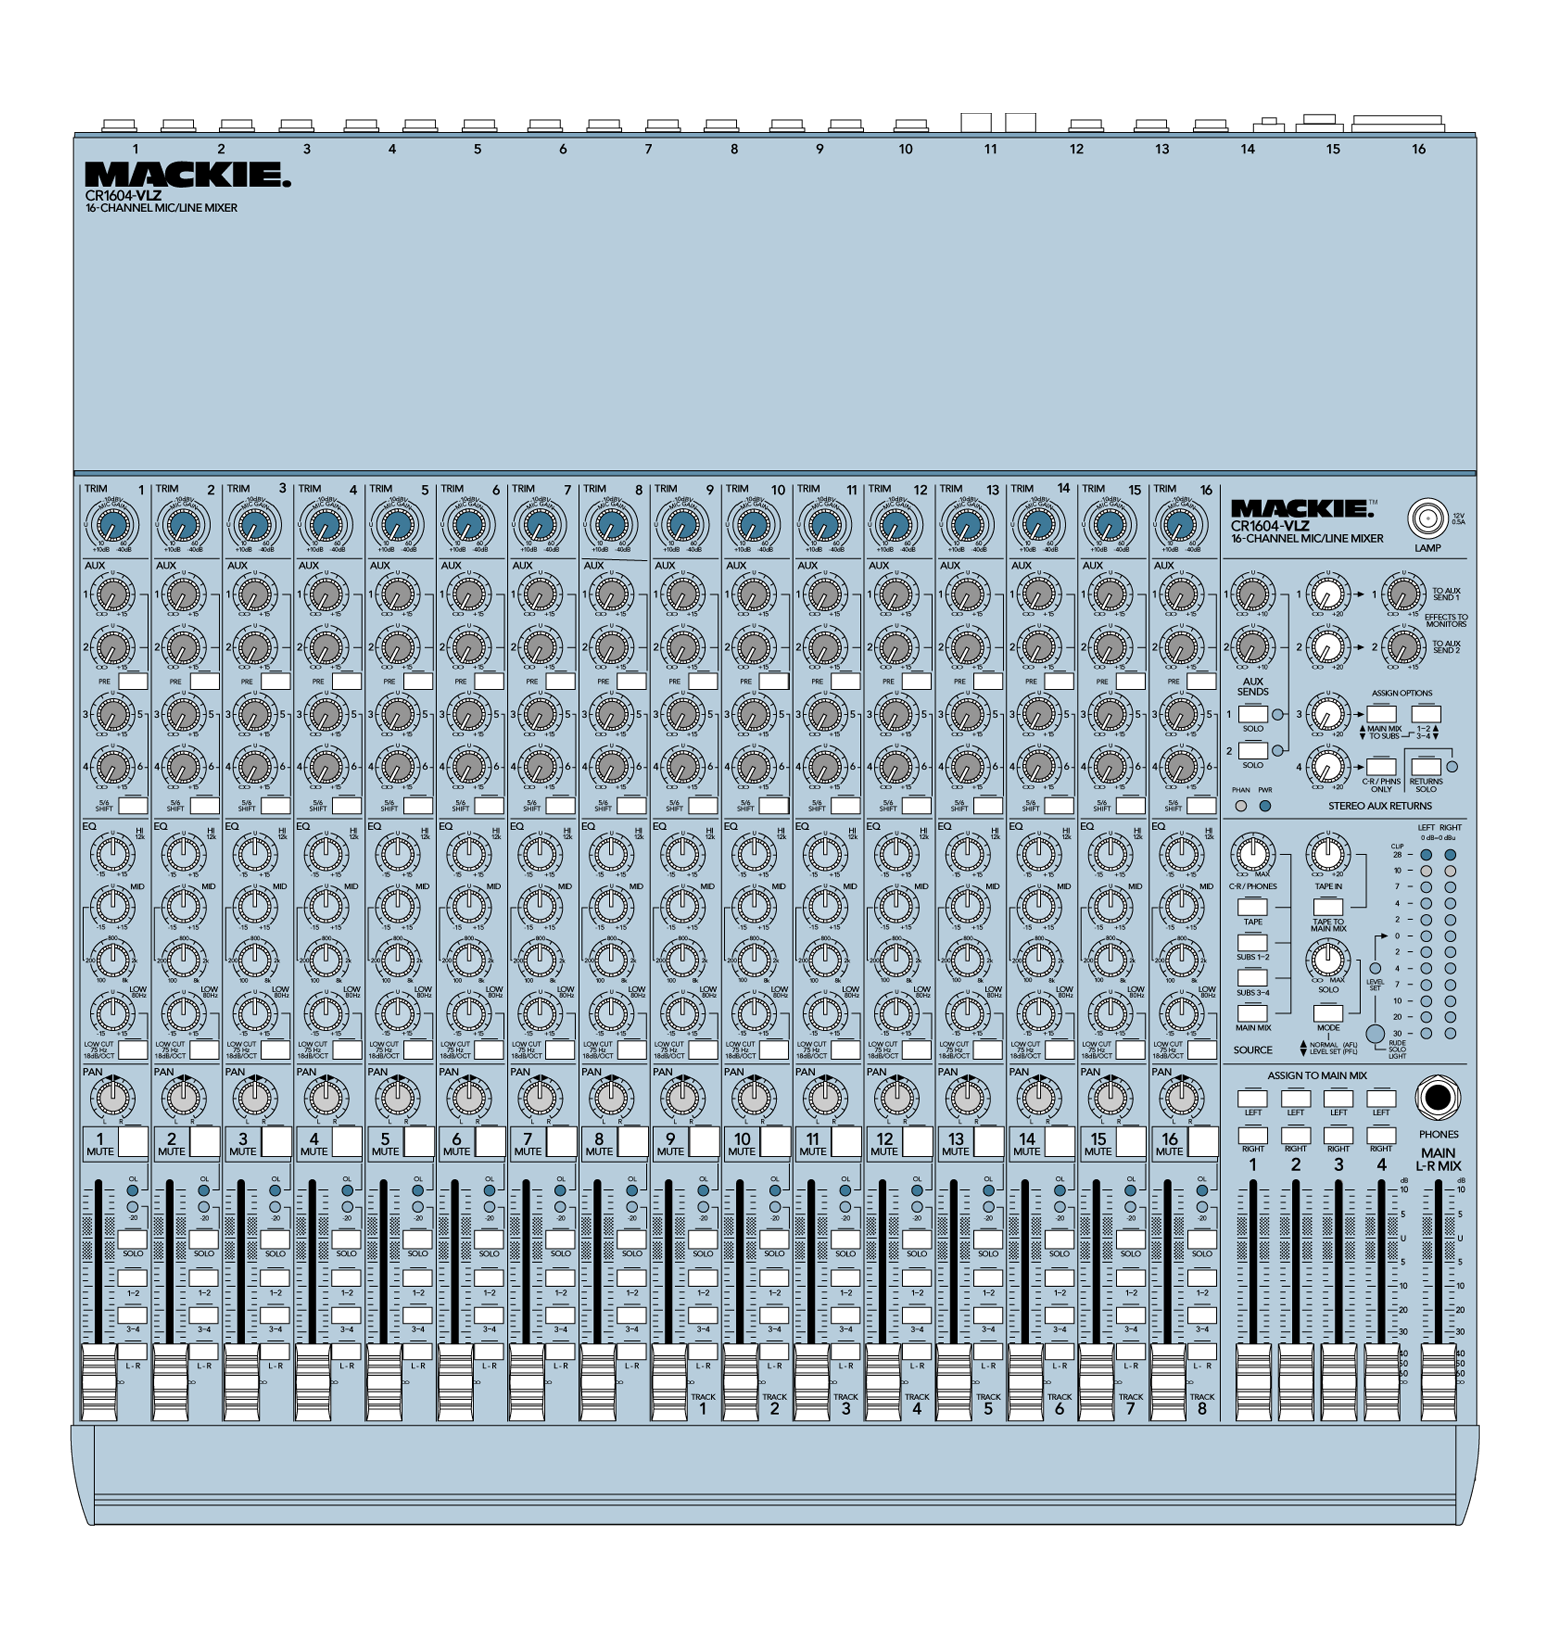
\includegraphics[width=.85\textwidth]{Mackie_Manual-1.png}
\caption{Mackie CR1604 Mixer}
\label{fig:fullfig}
\end{figure*}

\newpage

\begin{marginfigure}
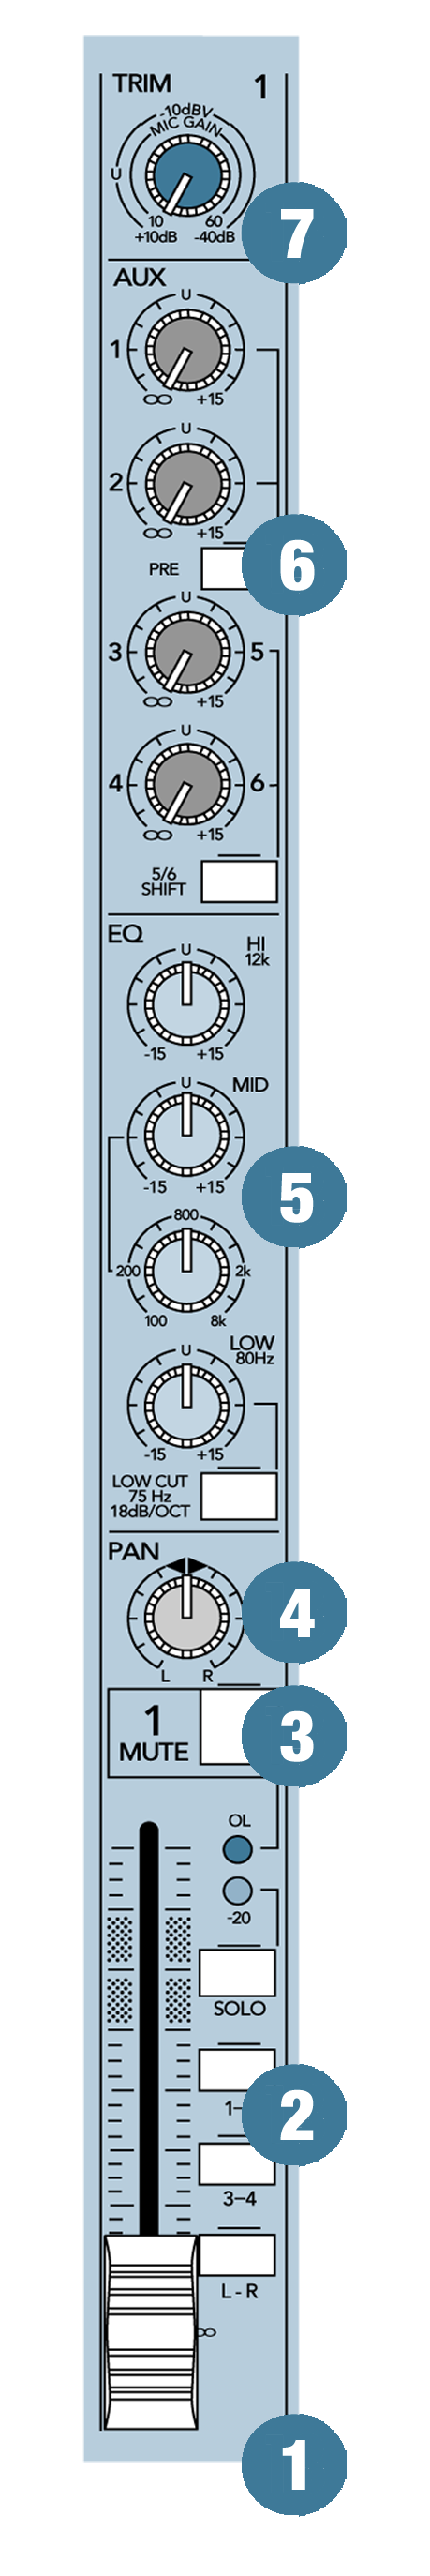
\includegraphics[width=\linewidth]{Mackie.png}
\caption{Channel from Mackie CR1604-VLZ Mixer}
\label{fig:marginfig}
\end{marginfigure}

\subsection{Controls of Individual Channel}

\begin{enumerate}
	\item Volume Fader: Controls the volume of the channel within the mixer
	\item Path (Subs): Chooses where the channel signal is directed to
	\begin{enumerate}
		\item \textbf{Solo}: Isolates the channel in the mix. Useful for when you only want to hear the specific channel without other ones. 
		\item \textbf{1-2}: Sends to Computer for Recording
		\item \textbf{3-4}: Sends to stereo $\frac{1}{4}$" cables for use with personal audio interfaces. 
		\item \textbf{L-R}: Sends only to Monitors (Speakers)
	\end{enumerate}
	\item Mute: Mutes the Channel 
	\item Pan: Controls the amount of signal sent to the left vs right, 1 vs 2, or 3 vs 4
	\item Equalization (EQ) 
	\begin{enumerate}
		\item \textbf{High EQ}: $\pm 15$ dB at $12$ kHz
		\item \textbf{Mid EQ}: $\pm 15$ dB within 1.5 octaves of the frequency center (Determined by Frequency Sweep) 
		\item \textbf{Frequency Sweep}: Selects the center of the Mid EQ between $100$ Hz and $8$ kHz 
		%\item \textbf{Low EQ}: $\pm 15$ dB at $80$ Hz 
		\item \textbf{Low Cut Switch}: Removes all signal below $75$ Hz (High Pass Filter) 
	\end{enumerate}
	\item Auxiliary Sends: Sends a parallel signal path to other outputs on the mixer. See \ref{fig:signal} for more information. 
	\begin{enumerate}
		\item \textbf{Aux A-B}: The DMV Pro effects processor has two inputs and can run different effects on each input. Aux \textbf{A} sends a signal to input 1 on the processor and Aux \textbf{B} sends a signal to input 2. See the section on the \hyperlink{effects processor}{effects processor}. 
		\item \textbf{Aux C-D}: Not used 
	\end{enumerate}
	\item Gain: Controls the amplitude of the signal going into the mixer. Input sensitivity is adjusted by $-10$ dB to $40$ dB. Please do not adjust unless necessary. 
\end{enumerate}

%------------------------------------------------

%\lipsum[1] 

\newpage

\subsection{Mixer}

\begin{marginfigure}
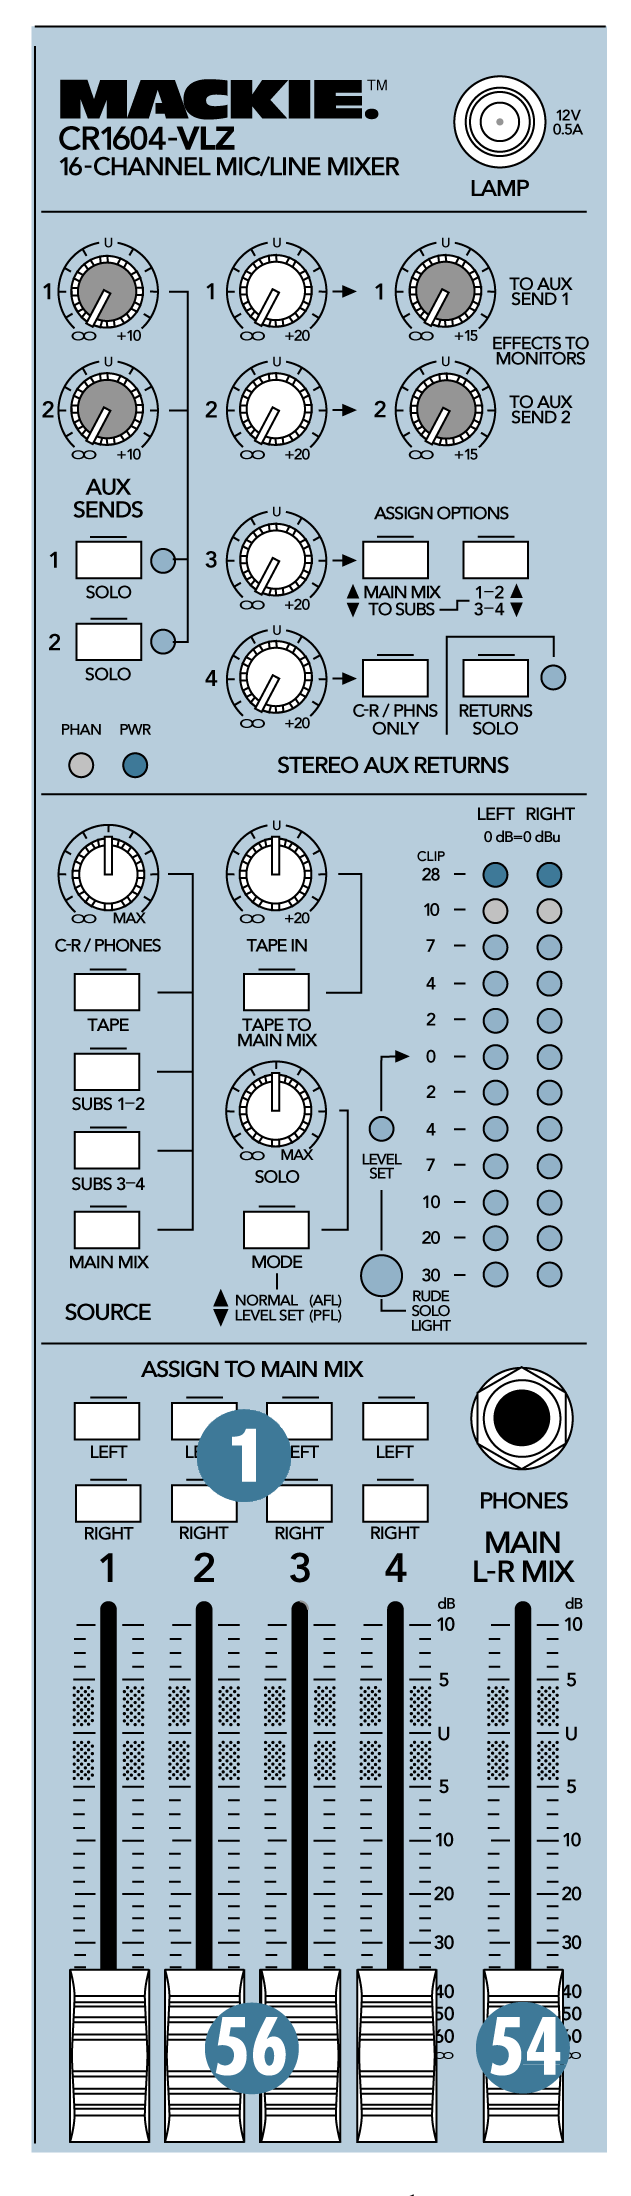
\includegraphics[width=\linewidth]{Mackie_2.png}
\caption{Master, Sub and Send Controls from Mackie CR1604-VLZ Mixer}
\label{fig:marginfig}
\end{marginfigure}

\begin{enumerate}
	\item Effects to Monitors: Adds effects to monitors. 
	\item Aux 1-2 Sends: Controls the gain of the AUX 1-2 send output into the mixer. 
	\item AUX Returns: Controls the volume of the signal returning from the AUX within the mixer. 
	\item 1-2/3-4 Toggles: Controls the path of the signal to 
	\item IGNORE ABOVE
	\item C-R/Phones: Controls volume to the Control Room out and the \hyperlink{Headphone Jack}{Headphone Jack}
	\item Selects what inputs are routed to the meter display
	\item Meter Display: Visually shows the strength of the signal. Want the highest possible signal strength (green) without clipping (red light). At yellow compression occurs.
	\item Selects what inputs are routed to the meter display, the C-R out and the headphone jack. 
	\item Solo Knob: Controls the level of the soloed channels
	\item Mode Control: 
	\begin{enumerate}
		\item \textbf{Normal (AFL)}: solo signal is post EQ, Pan, and Fader
		\item \textbf{Level Set (PFL)}: solo signal is pre EQ, Pan, and Fader
	\end{enumerate}
	\item \hypertarget{Headphone Jack}{Headphone Jack}: Accepts $\frac{1}{4}$ in. plug. Feel free to use your own headphones. 
	\item Main Mix Assigns: Allows fader subgroups 1-4 to be assigned left, right, or both channels in main mix. 
	\item Subgroup Volume Faders: Control the output levels of chosen group. Adjusting the volume of subgroup 1-2 will change the volume audio into the iMac. Adjusting 3-4 will change volume of the audio going into personal audio equipment. 
	\item Master Fader: controls output to speakers. 
\end{enumerate}








\newpage

\section{MIDI Time Piece MTP AV (MOTU)}
\subsection{Subsection 1}

\lipsum[9-10]

\subsection{Subsection 2}

\lipsum[11-12]

%----------------------------------------------------------------------------------------
%	CHAPTER 2
%----------------------------------------------------------------------------------------

\chapter{Chapter 2 Title}
\label{ch:2}

\lipsum[13-20]

%----------------------------------------------------------------------------------------

\backmatter

%----------------------------------------------------------------------------------------
%	BIBLIOGRAPHY
%----------------------------------------------------------------------------------------

\bibliography{bibliography} % Use the bibliography.bib file for the bibliography
\bibliographystyle{plainnat} % Use the plainnat style of referencing

%----------------------------------------------------------------------------------------

\printindex % Print the index at the very end of the document

\end{document}